\chapter{OMNeT++}
\label{cha:omnet}

OMNeT++ represents an open source simulation framework written in C++.
It provides an object oriented modular discrete event network simulation framework.
The platform independent simulation library includes an integrated development environment (IDE), which is based on the eclipse platform.
The commercial version OMNEST provides various licensing models, whereas OMNeT++ is only available for academic or non-profit use.
The intention of OMNeT++ is providing infrastructure for writing simulations for various fields; especially the field of network simulations.
For this thesis the current newest version of OMNeT++ 4.6 was used and analyzed.

Simulations developed with OMNeT++ are based on different components, which provide functionality for communication and topologies.

\section{Components}
\label{sec:omnet_components}
Within an OMNeT++ simulation different components are used to represent the simulated system.
Each component is described by a \emph{network description} (NED) file and can be enhanced with C++ code.
The \emph{NED} file contains information about the component which is necessary for connecting and designing the simulated system, such as gates, submodules and parameters.

The different types of components and their usage is explained in the next sections.

\subsection{Network}
\label{sec:omnet_components_network}
The outermost component is a network which consists of other components like modules and channels.
The simulated topology and the connections between modules are defined within the network.
A network represents a closed systems which can be simulated by itself, other components must be instantiated within a network to be simulated.
All instantiated modules, optional parameters and the connections between the modules are defined in the networks \emph{NED} file. \cite[section 3.2.1]{omnet_manual}

\subsection{Modules}
\label{sec:omnet_components_modules}
Modules represent functional groups of different complexities.
There are two types of modules available in OMNeT++.

A simple module is the smallest part within a simulated hierarchy and represents a functional unit.
For this functional unit the behavior for handling messages, the possible connections and additional parameters can be defined. \cite[section 3.3]{omnet_manual}
The possible connections of modules are represented by gates which can be connected to a channel or directly to other gates.

Multiple simple modules can be connected and be condensed to a compound module.
Such compound modules are used in the same way as simple modules, but represent bigger functional groups.
Compound modules are defined, in the same way as networks, the instantiated submodules and the connections between them. \cite[section 3.4]{omnet_manual}
For OMNeT++ a network and a compound module is the same component which differentiate by the value for the built in \emph{NED} property \emph{@isNetwork}.

An example network including simple modules connected to a compound module is shown in Figure \ref{fig:OMNeTComponents}.
Each module shown in Figure \ref{fig:OMNeTComponents} defines two gates which is either an input, output or bidirectional gate.

\begin{figure}
    \centering
    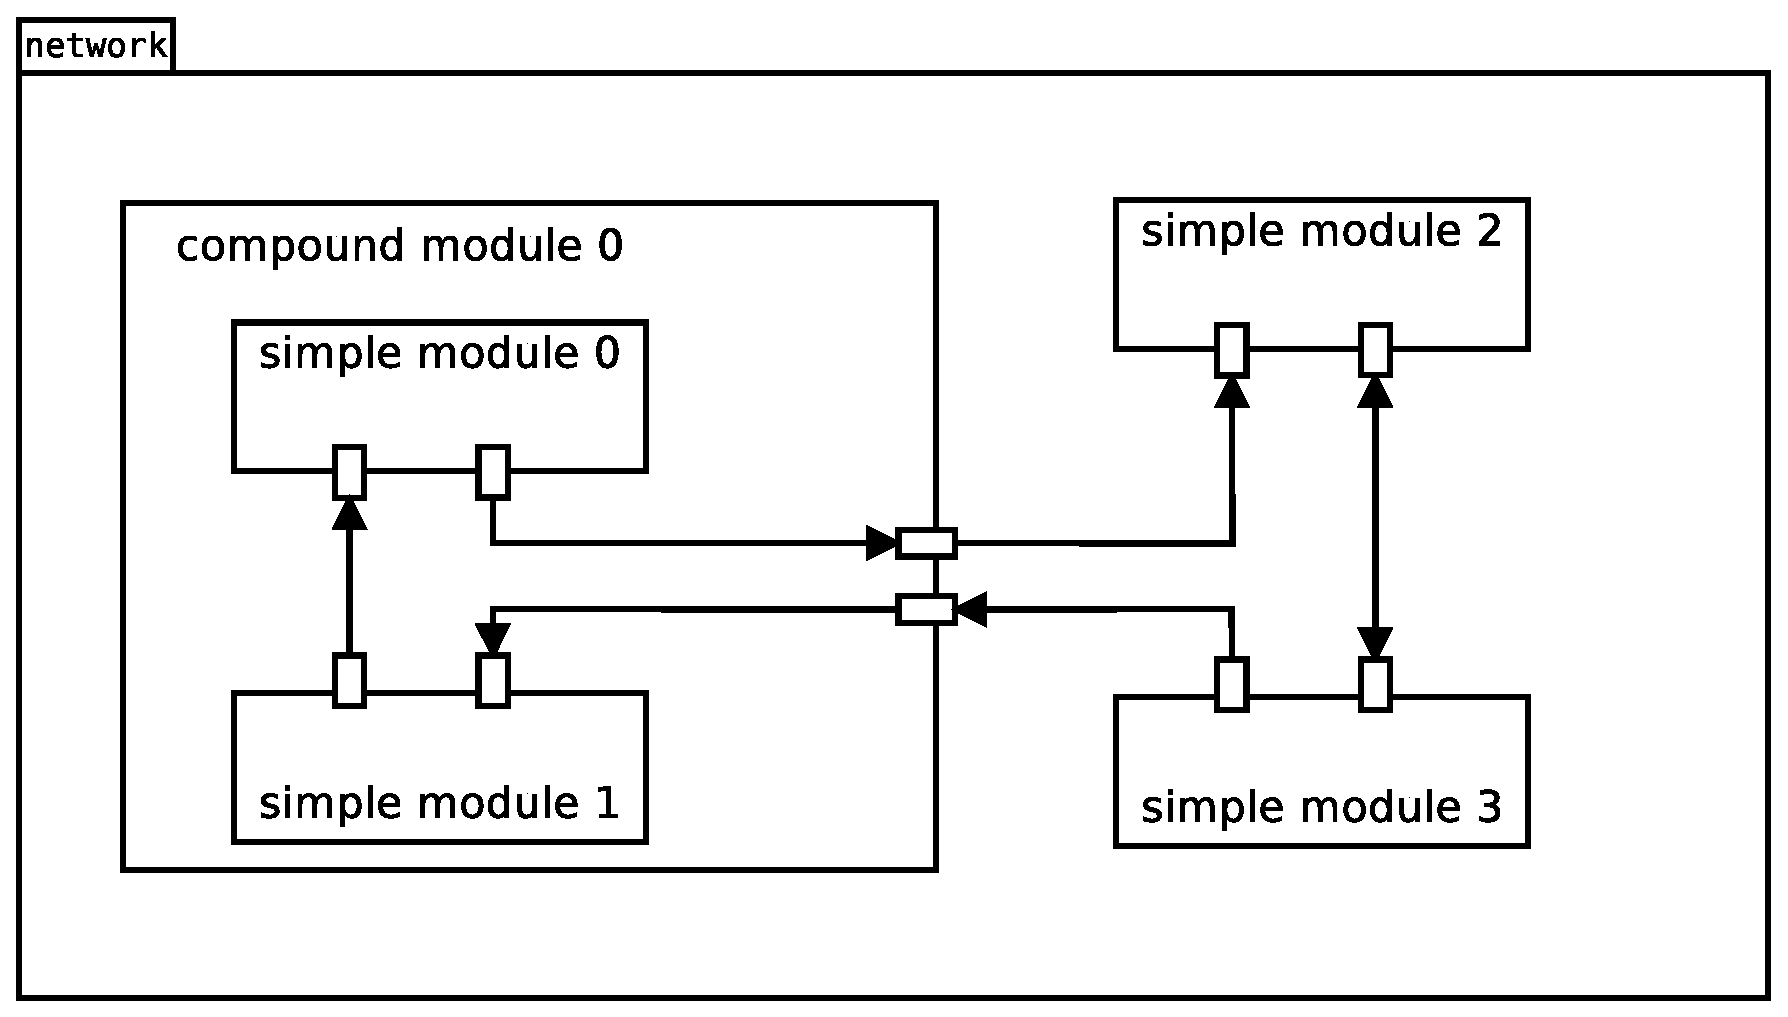
\includegraphics[width=0.9\columnwidth]{OMNeTComponents.eps}
    \caption{OMNeT++ components in an example network}
    \label{fig:OMNeTComponents}
\end{figure}

Specific functionality for custom components is implemented in the linked C++ code.
The assignment of \emph{NED} and C++ code is usually done with identical filenames, but can also be done manually with the \emph{@class} \emph{NED} property.
The components can embed any functionality implemented in C/C++.
The usage of external libraries or language features is not limited, but must be used with care due to the effect on simulation performance.
For implementing the behavior of the modules and accessing the simulation environment, for example reading the value of a defined \emph{NED} parameter or sending a message via a gate, 
OMNeT++ provides different functionalities and strategies.

The functionality of a compound module is given by the submodules and their connections.
A simple module is implemented by overriding specific methods following one of the two strategies below:

\begin{itemize}
    \item Using the \emph{handleMessage} method a module can react to incoming messages.
    Using this strategy the module is only active when a message is received.
    The methods \emph{send}, \emph{scheduleAt} and \emph{cancelEvent} can be used within \emph{handleMessage} for sending messages, scheduling self-messages and canceling of scheduled self-messages. \cite[section 4.4.1]{omnet_manual}
    
    \item The second strategy uses the method \emph{activity} and is also called \emph{process style} strategy.
    The method \emph{activity} is called by the simulation runtime as coroutine and can be implemented in the same way as a normal thread or process on an operating system.
    Returning from the \emph{activity} methods equals the finishing of the modules simulation.
    Beside the available methods of the first strategy, additional methods can be used within \emph{activity}.
    Using the method \emph{receive} the module waits until a message is received.
    Waiting a specific amount of simulation time is achieved with the \emph{wait} method.
    A simple module using the \emph{activity} method is called as coroutine of the simulation core and is scheduled non-preemptively.
    I.e. the activity method is not interrupted by the simulation and has to suspend by itself.
    This is done by waiting for a received message or waiting a specific amount of time. \cite[section 4.4.2]{omnet_manual}
\end{itemize}

\subsection{Channels}
\label{sec:omnet_components_channels}
The connections between modules can be realized in different ways.
A direct connection of two gates transports the transmitted messages immediately.
For applying transportation parameters (e.g. delay, latency, jitter) or implementing a custom behavior the connection can be established with a channel.
The OMNeT++ framework provides three built in channels for direct usage or sub classing.

\begin{itemize}
    \item The \emph{IdealChannel} represents the same behavior as a direct connection between gates and transmits each message immediately.
    \item The \emph{DelayChannel} provides a \emph{delay} parameter for configuring a constant delay for each message.
    Additionally there is the possibility to disable the channel and drop all containing messages.
    \item The \emph{DatarateChannel} provides the \emph{datarate} parameter for a variable rate of transmission including a configurable bit error rate (BER) and packet error rate (PER).
    These error rates can be used to mark a transmitted packet as erroneous.
\end{itemize}

These channels can be used directly or being subclassed for implementing custom functionality. \cite[section 3.5]{omnet_manual}

For implementing a custom Channel three Methods must be implemented:

\begin{description}
    \item[isTransmissionChannel] returns true if the channel is a transmission channel, i.e. the transmission duration is calculated and set within the packet.
    This type of channel only affects messages of type \emph{cPacket} or derived types.
    \item[getTransmissionFinishTime] returns the finish time of the transmission for messages of type \emph{cPacket} or derived types.
    \item[processMessage] models the behavior of the channel and its functionality.
    In this method the results can be stored in a provided structure, which allows a dropping of the message and a change of the resulting transmission time.
    The transmitted message is passed to the \emph{processMessage} method, therefore various modifications can be made simulating the transmission through the channel. \cite[section 4.8]{omnet_manual}
\end{description}

\subsection{Parameters}
\label{sec:omnet_components_parameters}
Each component can define various parameters for configuration of their behavior.
The value of these parameters can be assigned in different ways.
The assignment from a \emph{NED} file can be done directly, via inheritance, or via a compound module or network which contains the component.
All parameters can also be set via a configuration file (e.g. omnetpp.ini) or interactively requested from the user.
In the case of none assignment a parameter can also define a default value.

These parameters can be used by the implemented behavior by using the \emph{par} method. \cite[section 3.6]{omnet_manual}

\subsection{Messages}
\label{sec:omnet_components_messages}
Transmitted data is encapsulated in another component called message.
Messages are a fundamental component of an OMNeT++ simulation as they don't only transport data but can also represent functional messages like jobs, events or tasks.
The meaning of a message depends on the written simulation and the simulated system. \cite[chapter 5]{omnet_manual}

These messages can also be customized for holding a specific set of data like a protocol header, checksum, or other specific data.
The existing message class \emph{cMessage} and its derived specialization \emph{cPacket} provide different members and methods which can be used for simulations.
These include control information, type information, time stamp, etc. and are included to ease the development of a simulation.
Adding a few simple datafields to a message can be either done by subclassing \emph{cMessage}, \emph{cPacket} or using the \emph{NED} language in special \emph{.msg} files.
By defining a custom message using \emph{NED} a customized subclass will be generated by the simulation and can be used as normal Message. \cite[chapter 6]{omnet_manual}

Any module can send a message via its gates by using the \emph{send} methods or send it to itself as \emph{self-message} with \emph{scheduleAt}.
The mechanism of messages is also used for implementing timeouts, timers, etc. by sending a specific message to the current module.
Therefore the method \emph{scheduleAt} takes a absolute simulation and a message as parameters and sends the given message at the given point to the current module.
These \emph{self-messages} are handled by the same function as any other messages coming from other modules.
For the identification of \emph{self-messages} the built in method \emph{isSelfMessage} is available.
A scheduled \emph{self-message} can be canceled via the method \emph{cancelEvent} taking the scheduled message. \cite[section 4.7.1]{omnet_manual}

The \emph{send} methods takes the message to send and the used gate as parameter.
For defining the gate the defined name, the id or the object itself can be used. \cite[section 4.7.2]{omnet_manual}
When the transmission of the messages should occur at a later time, there is a built in functionality given with the \mbox{\emph{sendDelayed}} methods.
These methods work in the same way as the default \emph{send} methods but take an additional parameter which represents the delay. \cite[section 4.7.6]{omnet_manual}

Messages can also be sent directly to gates of defined modules without the need of a connection to the current module.
This is called \emph{direct sending} and can be useful when multiple sender modules send to a single input gate.
An example for this usage is shown in Figure \ref{fig:direct_sending}.

\begin{figure}
        \centering
        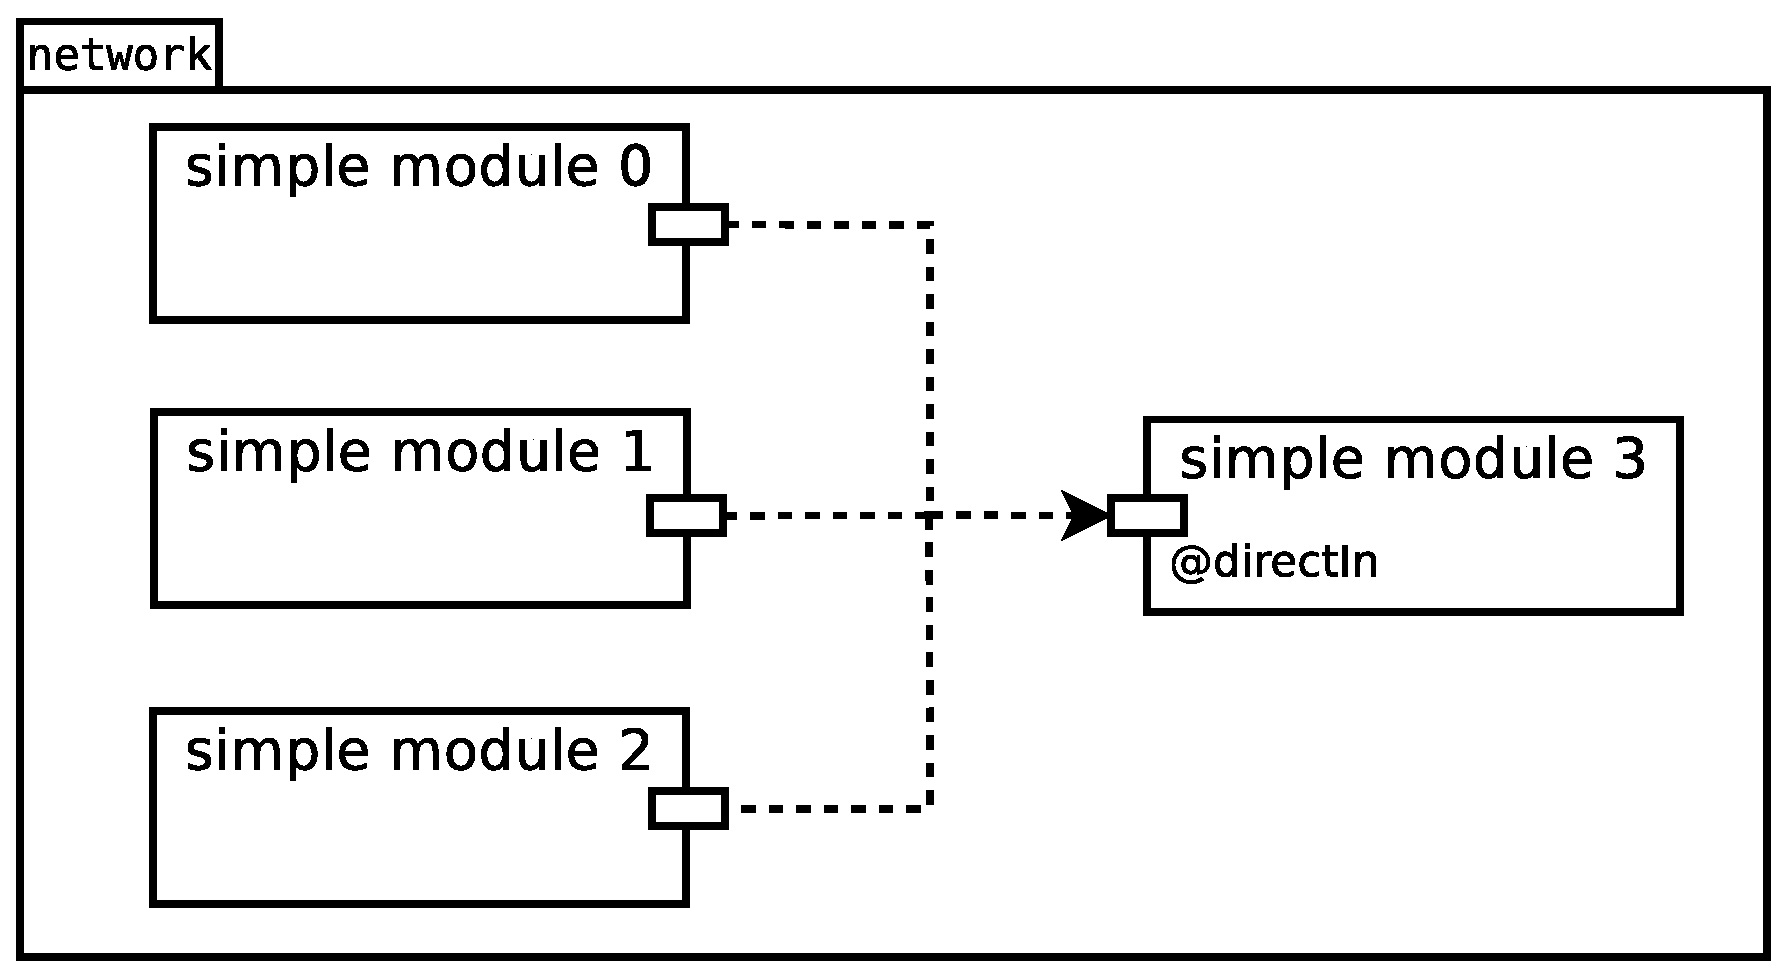
\includegraphics[width=0.9\columnwidth]{direct_message.eps}
        \caption{Multiple simple modules sending messages directly to simple module 3}
        \label{fig:direct_sending}
\end{figure}

Such a gate should be declared with the \emph{@directIn} \emph{NED} property to avoid notifications about a not connected gate. \cite[section 4.7.5]{omnet_manual}

Additional handling of messages as broadcasts and retransmission requires attention to the owner of messages.
By sending a message its owner changes to the simulation core and furthermore to the receiver module.
Therefore explicit copying of a message via \emph{dup} is necessary for sending a message to multiple modules or resending a message. \cite[section 4.7.3]{omnet_manual}

Each message sent either by another module or by the current module itself represents an event for the simulation with an according time, at which this event should happen, or the message should be delivered/received.
The execution and the handling of such events is done by the simulation core and defines the execution order and the performance of the simulation.
The different types of simulations and the simulation core of OMNeT++ is discussed in chapter \ref{cha:simulation}.


\section{Simulation results}
\label{sec:omnet_results}
The simulation of different systems results in different types of outcomes.
Therefore OMNeT++ provides multiple functionalities for recording and saving different results.


\subsection{Simulation library}
\label{sec:omnet_results_sim_lib}
The traditional way to record simulation results is using the simulation library functions.

The built in type \emph{cOutVector} provides the functionality used for recording a time series of data.
By holding an instance of \emph{cOutVector} a series of data can be recorded during simulation.
During initialization of the module the according name of the recorded time series should be set.
The recorded data of all \emph{cOutVector} instances is written at the end of the simulation to a single output vector file (\emph{.vec}). \cite[section 7.9.1]{omnet_manual}

Recording single values (scalars) is done using the \emph{recordScalar} method of a \emph{cModule}.
This mostly is called in the \emph{finish} method and may record a result of statistical analyze or even a whole statistic object.
All recorded scalars are written in a line based textfile (\emph{.sca}). \cite[section 7.9.2]{omnet_manual}

The recording and the format of single vectors or single scalars can be defined in a configuration file as described in section \ref{sec:omnet_results_config}.

This method leads to an increased dependency of result recording and the simulated system due to the hard-coded implementation.
Since OMNeT++ 4.1 the newer strategies using \emph{signals} and \emph{statistics} are available and provide alternative methods for results recording.

\subsection{Signals and statistics}
\label{sec:omnet_results_signals}
The idea behind result recording using signals and statistics is the separation of data generation and recording.
The generated data are represented and distributed via signals.
The statistics are accessing different signals for custom recording of required results. \cite[section 12.1.1]{omnet_manual}

Signals provide a functionality for a communication between modules which are not directly connected via their gates.
The usage of signals is following the \emph{publisher/subscriber} principle, i.e. modules can register callback objects to a specific signal.
If a new value for the signal is emitted all registered callback objects are notified.

Signals are defined in the \emph{NED} file of the according module or channel and can be accessed by the defined name of the signal or the resolved signal id.
The name of a signal is defined globally, i.e. signals with identical names in different modules represent the same global signal.
A registered listener of such a global signal receives notification of all modules which emit a new value for their signal. \cite[section 4.14]{omnet_manual}

Using the \emph{@statistic} \emph{NED} property the recording of data can be implemented using the built in functionalities.
By defining a statistic property to a signal, a filewriter listener will be registered which records all notifications on this signal.
A statistic property provides multiple functionalities and options which can be defined in the \emph{NED} file.

Declaring a simple statistic property creates a signal with the according statistic name.
For separated configuration of signal and statistic the \emph{source} option can be used to define a signal as the source of recorded data.
Built in filters provide existing functionality which can be directly embedded in the definition of the source signal.
For example the \emph{count} filter can be used to count the value notifications received on the defined signal.
Multiple filters can be chained for manipulating the receiving data.

The \emph{record} option defines what data shall be recorded by defining a recorder.
Recorders are the final elements of the recording chain, beginning at the source signal.
Between the source signal and the recorder a variable number of filters can be set.
A single statistic can define multiple recorders resulting in multiple recorded data.
For distinguishing the importance of recorders an optional question mark behind the recorder name can mark it as optional.
Optional recorders can be skipped by default, as described in section \ref{sec:omnet_results_config}.
The built in recorders like \emph{last}, \emph{min}, \emph{max}, etc. result in an output scalar.
The recorder \emph{vector} results in an output vector.
These generated output container represent the same functionalities as the traditional recording methods described in section \ref{sec:omnet_results_sim_lib}.

There are various built in filters and recorders available \cite[section 4.15.2]{omnet_manual} and there is also the possibility for writing and using custom filters and recorders. 
This can be achieved by subclassing \emph{cResultFilter} or \emph{cResultRecorder}. \cite[section 4.15.6]{omnet_manual}

The configuration of the resulting output (vector, scalar) is done independent of the used recording method.

\subsection{Configuration}
\label{sec:omnet_results_config}
The recorded results can be individually enabled and configured.
Therefore the configuration which data is recorded in which format is independent of the generated results and can be configured via a configuration file (\emph{.ini}).

The recording using signals and statistics provides more options and possibilities and require therefore more different configuration methods.
Each statistic object can be configured individually using the \emph{result-recording-modes} for each statistic defined by its full path within the hierarchy.
This option defines the enabled recording modes (recorders described in section \ref{sec:omnet_results_signals}).
Additionally to the available recorders the presets \emph{default} and \emph{all} are available.
The \emph{default} set contains all non-optional recorders, i.e. all recorders excluding recorders marked with a question mark.
The \emph{all} set contains all non-optional and optional recorders. \cite[section 12.2.1]{omnet_manual}

Statistics based recording consider a defined warm-up period which can be defined via \emph{warmup-period}.
Within this time beginning from the start of simulation no statistics will be recorded.
When using the simulation library to manually record results (cOutVector, recordScalar) the warm-up period must be considered manually. \cite[section 12.2.2]{omnet_manual}

The resulting output files can be defined independently of the used recording method via the options \emph{output-vector-file} and \emph{output-scalar-file}. \cite[section 12.2.3]{omnet_manual}

The configuration of the recording via the simulation library (section \ref{sec:omnet_results_sim_lib}) is done by \emph{scalar-recording}, \emph{vector-recording}, \emph{vector-recording-interval} and \emph{vector-record-eventnumbers}.
These options allows the dis- or enabling of specific output vectors and scalars given by their full path within the hierarchy.
For vector recording the definition of specific recording intervals is possible to record only interesting intervals.
Also the addition of the event number to the output file can be dis- or enabled.
These options also affect the recording via signals and statistics because the statistic property generate output vectors and scalars. \cite[section 12.2.4, section 12.2.5]{omnet_manual}

\section{Running an OMNeT++ simulation}
\label{sec:omnet_running}

The output of the OMNeT++ build process is by default an executable for starting the simulation.
All generated simulation executables provide command line parameters for the configuration of specific simulation runs.
The most important parameter can be passed directly or via the \emph{-f} command and defines the used configuration files for the simulation run.
The configuration files and some key options for running a simulation is described in section \ref{sec:omnet_running_config}.

Within a configuration file multiple configurations can be defined and the configuration which should be used for simulation can be defined via the \emph{-c} command line option.
If no configuration to load is specified but multiple configurations are defined within the configuration file the behavior depends on the started user interface.
Starting the graphical user interface will prompt the user to choose a configuration.
The command line user interface will execute the general configuration.

The configuration of the path to load the \emph{NED} files can be defined within a configuration file as well as by a command line option (\emph{-n}).
With multiple configurations the values are merged into a combined load path.

The selection of the user interface can be defined via the command line option \emph{-u}.
This define overrules a configured default user interface of a configuration file.
The different user interfaces and their functionalities are shown the sections \ref{sec:omnet_running_tkenv} and \ref{sec:omnet_running_cmdenv}.

OMNeT++ also provides the \emph{oop\_run} tool, which is basically an empty simulation.
With this tool a simulation model which is built as shared library can be started.
With \emph{oop\_run} or any other simulation executable all available command line options and their description are acessable via \emph{-h}.

Further configuration options of the configuration file can also be set via the command line interface by preceding the option with \emph{-{}-}.
In case of double configuration the via command line parameter passed value will be preferred. \cite[section 10.1.1, section 10.1.2]{omnet_manual}

\subsection{Configuration}
\label{sec:omnet_running_config}
The configuration file can be given by a command line parameter, usually the file \emph{omnetpp.ini} is used.

Within a configuration file multiple configurations or sections can be defined.
When starting a simulation the loaded configuration can be set, therefore multiple different simulation runs with different configurations can be defined within a single configuration file. \cite[section 9.2]{omnet_manual}

The most essential configuration is the simulated network which is defined by the name of the according \emph{NED} network.

The duration of the simulation can be defined via an ending simulated system, i.e. modules which automatically finish their execution, or a time limit is defined.
A time limit can either be defined for the simulation time (\emph{sim-time-limit}) or the cpu time (\emph{cpu-time-limit}).

The behavior of the simulation in case of errors and the connection behavior of debuggers can be defined via various options as \emph{debug-on-errors}, \emph{debug-attach-on-error}, etc.. \cite[section 10.1.3]{omnet_manual}

Specific configuration for the command line user interface are available for controlling the output of a running simulation (\emph{cmdenv-express-mode}, \emph{cmdenv-status-frequency}, \emph{cmdenv-perormance-display}) and the possibility of user interaction (\emph{cmdenv-interactive}).
The effects of these options are shown in section \ref{sec:omnet_running_cmdenv}.

Parameters of loaded components can be set individually, commonly set via wildcards, or requested from the user.
Values which are directly set within the \emph{NED} files can not be overwritten by a configuration file.
Therefore a more flexible simulation model provides the majority of parameters via configurations.
Parameter of modules can either be set individually by the full path within the simulated hierarchy or commonly set via wildcards. \cite[section 9.3]{omnet_manual}

The configuration of module parameters also allow the definition of value ranges for so called \emph{parameter studies}.
These \emph{parameter studies} result in multiple simulation runs iterating over all specified parameters.
Simulating a specific iteration can be achieved via setting the run number passed by command line interface (\emph{-r}) or defined in the configuration (\emph{cmdenv-runs-to-execute}. \cite[section 9.4]{omnet_manual}

Defined via the command line parameter or via the \emph{user-interface} option different user interfaces can the used to start and visualize the simulation.

\subsection{Graphical user interface \emph{Tkenv}}
\label{sec:omnet_running_tkenv}
OMNeT++ provides the graphical environment \emph{Tkenv} for running and visualizing simulations.
\emph{Tkenv} provides various different possibilities for a graphical presentation of the simulated network, processed events and simulation results.

This user interface is useful for developing and debugging a simulation during the development.
The possibilities to inspect each component within the simulated system provide deep insight in the simulated system.

Different possibilities for graphical representation of the system and animation of progress/results allow a convenient presentation of a simulated systems.
This presentation allows educational and presentational purposes of the simulation. \cite[section 7.1]{omnet_user_guide}

Running complex simulations with multiple parameter studies is not recommended within Tkenv due to the increased overhead for refreshing the representation.
Different run modes (\emph{normal run}, \emph{fast run}, \emph{express run}) allow the skipping of user interface updates. \cite[section 7.3.2]{omnet_user_guide}

For simulations with increased complexity and longer simulation durations the command line user interface \emph{Cmdenv} should be preferred.

\subsection{Command line user interface \emph{Cmdenv}}
\label{sec:omnet_running_cmdenv}
The \emph{Cmdenv} environment represents a command line user interface.
Using this environment no graphical user interface is shown, or will be updated.
This simulation method is recommended for batch simulations or running simulations with increased complexity and no need for graphical representation due to the improved performance.

During a running simulation within \emph{Cmdenv} the output printed to the command line depends on the configuration.
For debugging purposes the \emph{normal mode} can be used and detailed event information will be printed to the command line.
Running simulations over a longer period of time the \emph{express mode} is recommended and only periodically status updates will be printed.
The frequency of the updates and the printed details can be configured via the \emph{cmdenv-status-frequency} and the \emph{cmdenv-performance-display} options. \cite[section 10.2.3]{omnet_manual}

Simulations defining one ore more parameter studies result in multiple runs which can be defined via a command line parameter or in the configuration.
For executing multiple runs OMNeT++ provides the \emph{oop\_runall} tool which starts each run in a separate operating system process.
Using multicore/multiprocessor systems \emph{oop\_runall} can execute different simulation runs on different cores/processors. \cite[section 10.4.3]{omnet_manual}
\\

Running the simulation within \emph{Tkenv} or \emph{Cmdenv} executes it by default sequentially.
Parallel simulation imposes different requirements on the simulated systems and its design.
These requirements and the functionality of parallel simulation is analyzed in chapter \ref{cha:parallel_sim}.

\section{Simulation Core}
Simulations based on OMNeT++ are designed and simulated as discrete event simulations (\emph{DES}).
The characteristics of the \emph{DES} and the comparison to other types of simulation are discussed in the next chapter \ref{cha:simulation}.

Details about the different simulation properties and functionalities are examined in section \ref{sec:simulation_omnet}.